%knowledge-flows.tex
\documentclass[12pt]{article}
\usepackage{amssymb,latexsym}
\usepackage[round,sort]{natbib}
\usepackage{multirow,array}
\usepackage{fancyhdr}
\usepackage{lastpage}
\usepackage{graphicx}
\usepackage[bottom]{footmisc}
\graphicspath{ {knowledge-flows-images/} }
\usepackage[T1]{fontenc}
\usepackage{mathptmx}
\usepackage{tabu}
\usepackage{textcomp}
\usepackage{stata}
\usepackage{listings}
\usepackage[a4paper]{geometry}
\usepackage{hyperref}
\hypersetup{
    colorlinks=true,
    linkcolor=blue,
    filecolor=magenta,      
    urlcolor=cyan,
    citecolor=magenta,
}
\geometry{
 total={150mm,247mm},
 left=25mm,
 top=25mm,
}
\lstset{
basicstyle=\ttfamily,
columns=flexible,
breaklines=true
}
\newenvironment{hypothesis}{
  	\itshape
  	\leftskip=\parindent \rightskip=\parindent
  	\noindent\ignorespaces}

\pagestyle{fancy}
\fancyhf{}
\lhead{Heterogeneity in knowledge flows across regions}
\rfoot{Page \thepage  \ of \pageref{LastPage}}
\rhead{Iyenggar}

\begin{document}
\title{Heterogeneity in knowledge flows across regions:\\  Investigating patterns and mechanisms}
\author{Ashwin Iyenggar  (1521001) \\ ashwin.iyenggar15@iimb.ernet.in} 


\maketitle
\thispagestyle{empty}

\begin{abstract}
We analyze the pattern of knowledge flows by geographical region and by firm for seven prominent regions. We demonstrate that locations display significant heterogeneity with regard to the relative proportions of local and non-local knowledge flows, and within firm and across firm knowledge flows. Specific patterns idiosyncratic distribution of flows are identified by location and suggestions are made for furthering of theory on the causal contributors of knowledge flows.
\end{abstract}

\section{Introduction}\label{S:Introduction}
The agglomeration characteristics of economic regions have been highlighted by scholars since long\citep{Marshall1890}. More recently, scholars have demonstrated through numerous studies that patent citations provide a paper trail of evidence for the existence the knowledge spillovers in economic regions \citep{Jaffe1993, Almeida1999},  the effects of inventor mobility (e.g., \cite{Almeida1999}), of Intellectual Property Rights regime of locations (e.g., \cite{Zhao2006}) and of the role of international geography (e.g., \cite{Singh2007}) on knowledge spillovers. Knowledge spillovers is observed in practice however, to be highly heterogenous across locations, firms and legal regimes. The question of the causal mechanisms leading to knowledge spillovers remains largely unresolved, despite the enormous progress made by prior scholars. In this article, we investigate the patterns of knowledge flow as evidenced by patent citations across geographic regions around the world and use our findings to ascertain plausible causal factors leading to the heterogeneity in knowledge flows.
\\\\\
Literature in the strategy area has highlighted the importance of innovation as a source of competitive advantage in firms. Scholars have highlighted that firms have tended to adopt two distinct strategies in seeking to capture greater advantages in knowledge flows: a) geographic clustering \citep{Porter2003}, and b) the globalization of R\&D \citep{Almeida1996}. Scholars have in the past conclusively demonstrated that the bay area in California  demonstrates strong  cluster characteristics in that there are strong flows of knowledge within and across firms from within the same geographical area. While the benefits to such geographical localization of knowledge flows \citep{Porter2003} has been celebrated as an important aspect of the superior economic performance of Silicon Valley, there has been little work that has explored the same for  emerging innovation regions of Bangalore, Beijing, Israel and Austin. In this article, we analyze the nature of knowledge flows at the level of the region in aggregate rather than focus on specific industries of technologies as have been done in past studies \citep{Lecocq2016}.  In order to understand if these emerging innovation regions are trending toward clustering \citep{Jaffe1993} or globalization or knowledge flows or both, we categorize all knowledge flows along two dimensions\footnote{I am grateful to Prof. Sai Yayavaram for having proposed this framework as being an appropriate one for analyzing patent flows. To him should go the credit for much of the ideation and structure of this project. I however, singly own the responsibility for errors and omissions}: a) as a relationship between the geographic region of the creator of the knowledge and the geographic region of the user of the knowledge, and b) as a relationship between the firms that create the knowledge (assignee of the cited patent) and those that use the knowledge (assignee of the citing patent). This classification allows us to see knowledge flows in four mutually exclusive but collectively exhaustive categories as illustrated in Table ~\ref{table:matrix}\\

\begin{table}
\begin{centering}
\caption {Categories of Knowledge Flows}
\label{table:matrix}
\begin{tabular}{c|c|c|c|}
\multicolumn{1}{c}{}&\multicolumn{1}{c}{}&\multicolumn{2}{c}{Geographic Region}\\
\cline{2-4}
&&{Same}&Different\\
\cline{2-4}
\multirow{2}*{Assignee}&{\rotatebox{90}{Same}}&{\hfill Independent Research Centre}&{\hfill Geographic Diversification}\\
\cline{2-4}
&{\rotatebox{90}{Different}}&{Cluster}&{Diffusion}\\\cline{2-4}
\end{tabular}
\end{centering}
\end{table}

\noindent In Table ~\ref{table:matrix}, the quadrants on the left column indicate knowledge flows within the region whereas the quadrants in the right column indicate knowledge flows to other regions. We are  interested in understanding if the emerging innovation clusters of Bangalore, Beijing, Israel, and Austin show the characteristics of  geographical clustering \citep{Jaffe1993}. We use the Boston region and Silicon Valley as  leading innovation clusters to inform our reference point in studying the emerging innovation clusters.
\\\\
The investigation of potential mechanisms behind local spillovers is interesting for a number of reasons. Given the wide disparity in the extent of knowledge spillovers across locations, across firms and across IPR regimes it is intriguing to a researcher to find the mechanisms that may lie behind such a phenomenon. A specific flavor of this question is the investigation of the spillover effects of patenting in emerging countries, or those known to have weaker IPR regimes. Specifically, do multinational firms that develop patentable technologies in emerging countries create spillover effects in the host country talent pool, or do the benefits remain localized to within multinational companies (MNCs)? From a policy perspective, it is valuable to understand the impact of allowing MNCs dominate the patenting process in emerging markets on the quality of the talent pool in the host country. Does a significant group of local inventors develop? Is this affected by the strength of the IPR regime in the host country? Patents data allows us to ask and try and answer this question. 
\\\\
We evaluate the nature of knowledge flows across geographic regions by initially looking at six major regions of the world: San Francisco and greater Bay Area of California, Austin, Texas, the greater Boston area, Tel Aviv, Beijing and Bangalore. The sampling has been made keeping in mind both established and upcoming technological locations. 

%\section{Hypotheses}

%\begin{hypothesis}
%{\\Hypothesis 1: San Francisco and San Jose will have higher local flows than Bangalore\\}
%\end{hypothesis}

\section{Methods}
\subsection{Unit of Analysis}
Our unit of analysis is the flow of knowledge between locations, between assignees. In order to proceed with empirical work, we make the following decisions.  First, we focus our analysis on a region of interest, and flows are observed over time. Second, we map flows onto the two dimensions of region (geography) and assignee. Along each axis we are interested in local and internal flows as against global and external flows of knowledge. Finally, in order that the various regions may be compared on these axes, the flows of knowledge within each quadrant will be normalized to a percent value of the total flows for that region that year. 

\subsection{Definition of Geographic Regions}
We discuss here how we go about defining the geographic regions of interest to this investigation.  For locations in the United States, it is standard to use Metropolitan Statistical Areas (MSA) for analyses related to economic geography. The approach is less standard for non-US locations, and this problem is particularly exacerbated by the absence of a similar measure as the MSA. Urban areas are a reasonable substitute for  economic centers, and we therefore determine to use one such definition. Specifically, for MSA of US locations, we obtain data from \href{http://www.census.gov/geo/maps-data/data/cbf/cbf_msa.html}{the US census} and for urban areas for world wide locations, we obtain data from \href{http://www.naturalearthdata.com/downloads/10m-cultural-vectors/}{Natural Earth Data}.
\\\\
This automatically raises conflicting definitions for locations in the United States. So that the MSA definitions take precedence, we eliminated all data pertaining to US locations from the Natural Earth urban centers data and integrated this with the MSA information. With this we  generated a single database of location information for economic centers around the world. The appendix provides visual map-based snapshots of our regions of interest. The regions colored yellow are the ones in focus, while those in purple are neighboring regions outside the region of interest. 
\\\\
We note from the MSA data that the Bay Area of California is actually split between the two MSA regions of San Francisco-Oakland-Hayward, CA and San Jose-Sunnyvale-Santa Clara, CA. we therefore decide to treat the two as two regions for the current analysis. It is possible that we may need analyze the data again clubbing the two in the future. Bangalore is seen as including Hosur, the Boston-Cambridge-Newton MSA includes parts of New Hampshire and Beijing seems to extend a bit to the south.  These seem to be reasonable definitions for the respective economic geographies. 
\begin{table}
\begin{centering}
\caption {Categories of patent citations}
\label{table:uspatentcitation}
\begin{tabular}{|c|c|}
\hline
\textbf{Category}&\textbf{Number of citations}\\\hline
cited by applicant&16,527,942\\\hline
cited by examiner&17,174,252\\\hline
cited by other&25,444,463\\\hline
cited by third party&325\\\hline
&21,581,784\\\hline
\end{tabular}

\end{centering}
\end{table} 

\subsection{Mapping geographical co-ordinates to regions}
The file named \verb|location.tsv| from patentsview.org contains the latitude and longitude information for all locations referenced in the patentsview.org database. The \verb|location.tsv| associates a \verb|location_id| to each latitude-longitude combination. we use the merged MSA and urban centers information and the geographical information in \verb|location.tsv| to obtain a mapping from each \verb|location_id| used in the patentsview database to the economic geography that it corresponds to. The patentsview.org database defines 128,911 unique location\_ids, and our data is able to map 53,424 of those locations to an economic geography region. The rest are assumed to be those locations that fall outside any major urban center in the world from which patents from been filed or been assigned.

\subsection{Selecting applicant cited patent citations}
The \verb|uspatentcitation.tsv| file from patentsview.org maps every patent-patent level citation that has been made since 1976. This file has 80,728,766 observations. Table ~\ref{table:uspatentcitation} provides a break up based on category. The US patent office has been systematically categorizing citations by category since after the year 2000. This explains the many empty citation category entries. 
\\\\
In order that we are consistent with our initial objective of measuring only applicant cited patents as flows of knowledge, we restrict ourselves to those patents categorized as 'cited by applicant'. This decision has the additional effect of limiting our period of analysis to citing patents applied for after the year 2000. 
\begin{table}
\begin{centering}
\caption {Number of citation entries by region of interest (till 2012)}
\label{table:selected-citations}
\begin{tabular}{|c|c|}
\hline
\textbf{Region}&\textbf{Number of citations}\\\hline
Boston-Cambridge-Newton, MA-NH&4,602,355\\\hline
San Jose-Sunnyvale-Santa Clara, CA&8,431,536\\\hline
Bangalore&183,685\\\hline
Beijing&131,752\\\hline
Tel Aviv-Yafo&872,578\\\hline
San Francisco-Oakland-Hayward, CA&9,258,684\\\hline
Austin-Round Rock, TX&259,503\\\hline
\end{tabular}

\end{centering}
\end{table}

\subsection{Expanding the US patent citation}
We use the \verb|application.tsv| file to determine the year of application of the citing patent and then use this to add a year field to the uspatentcitation entry. After selecting only those citation entries where the year of application of the citing patent is 2012 or earlier, we are left with 11,822,154 citation entries. In order to determine internal firm flows or external firm flows of knowledge, we use the assignee\_id on each patent to identify similarity or dissimilarity of assignees. There are 5,300,888 unique assignee entries. While a vast majority of patents are assigned to a single assignee, there are a few that are assigned to more than one assignee. In attaching assignee\_id to each citing and cited patent on a citation, we create separate entries for each unique assignee on each patent. With this we end up with 12,256,759 citation entries of which 2,869,978 entries have an empty assignee\_id for either the citing patent or the cited patent. A future revision could potentially work to reduce the loss due to empty assignee\_id. The 12,256,759 citation entries with year and assignee\_ids for both citing and cited patents are then expanded to include every inventor on each citing patent and each cited patent. This process is performed using a Python script as the joinby process was turning out to be extremely time consuming on \stata \ (we had runs of over 40 hours without \stata \ finishing). At the end of this process, we had 105,369,401 citing-patent-assignee-location to cited-patent-assignee-location citation entries. This formed the master dataset for the further analysis.


\begin{figure}[h]
\begin{centering}
  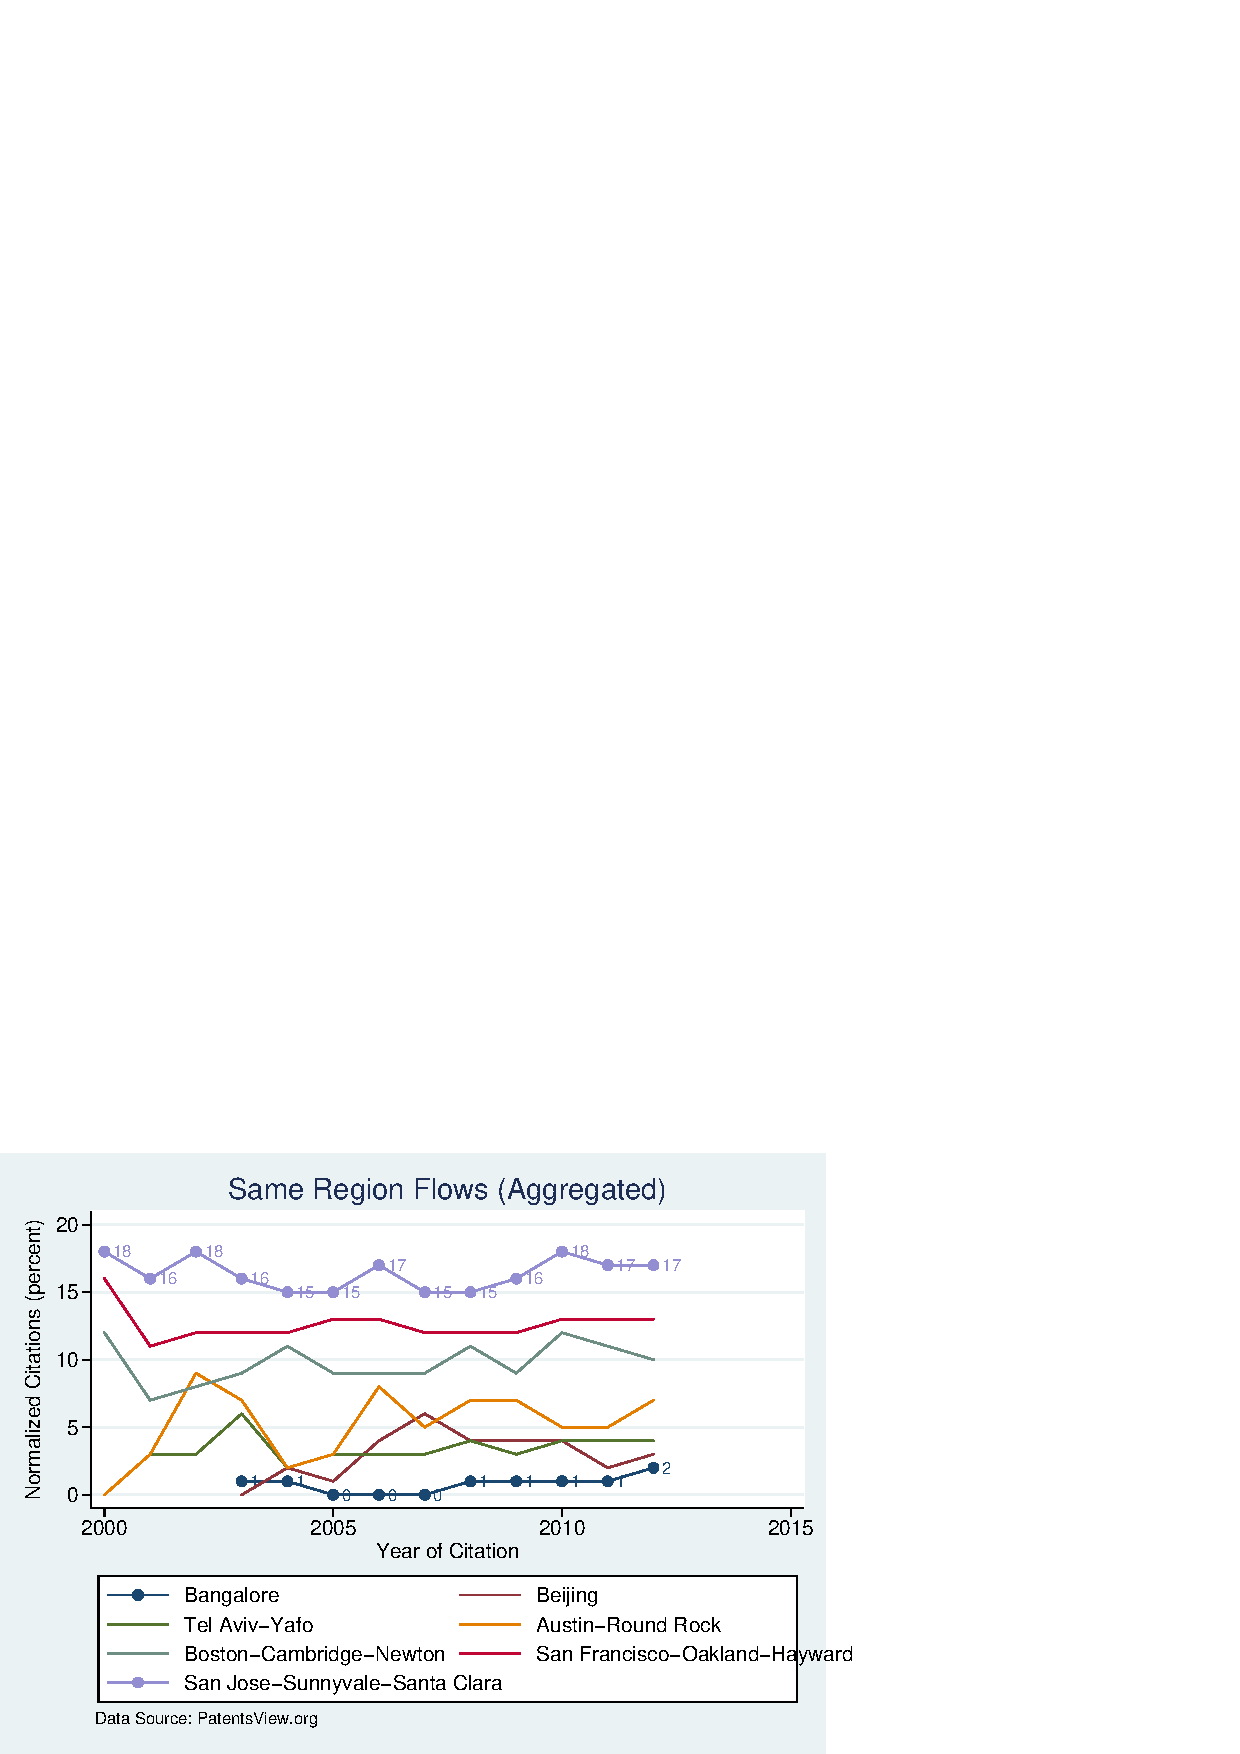
\includegraphics[width=\textwidth]{SameRegionFlows}
  \caption{Local Knowledge Flows by Region}
  \label{fig:SameRegionFlows}
\end{centering}
\end{figure}

\begin{figure}[h]
\begin{centering}
  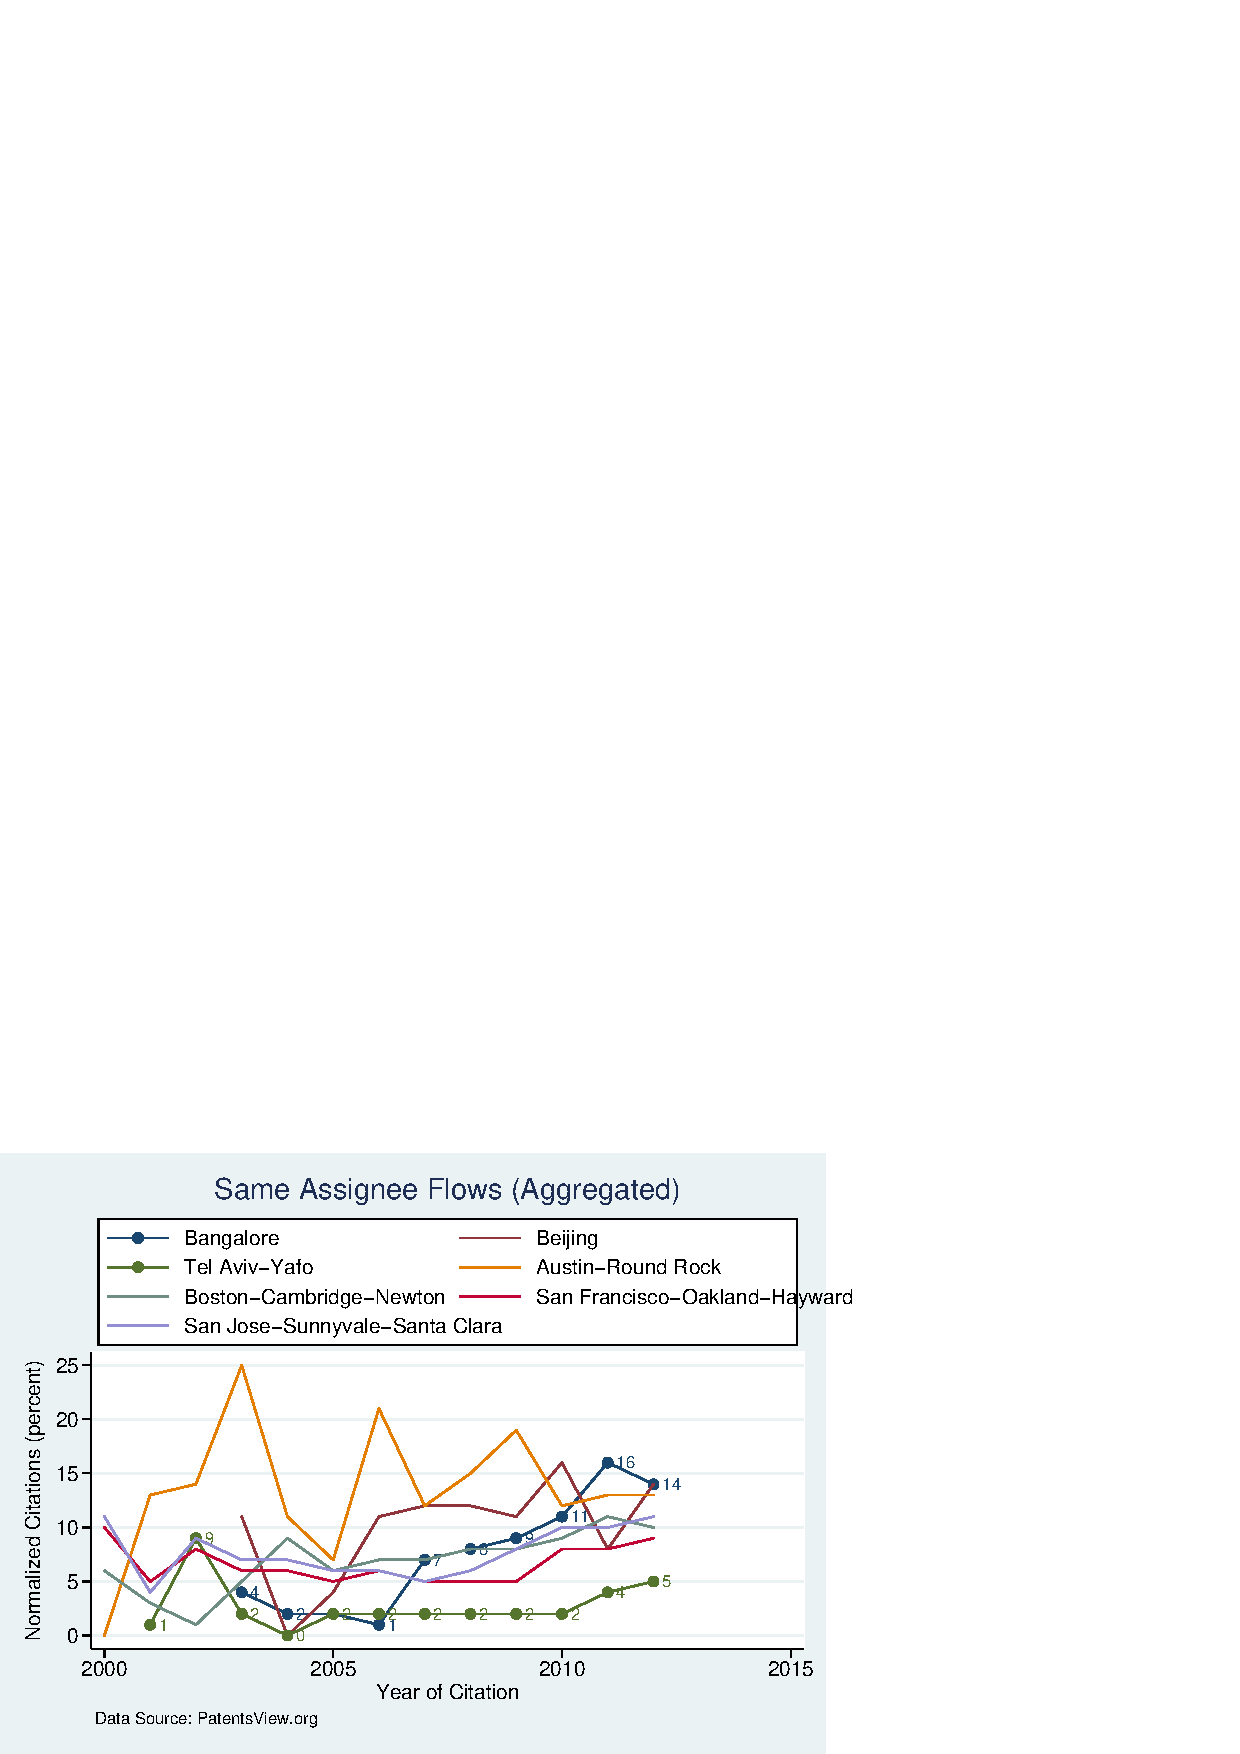
\includegraphics[width=\textwidth]{SameAssigneeFlows}
  \caption{Internal Knowledge Flows by Region}
  \label{fig:SameAssigneeFlows}
\end{centering}
\end{figure}


\begin{figure}[h]
\begin{centering}
  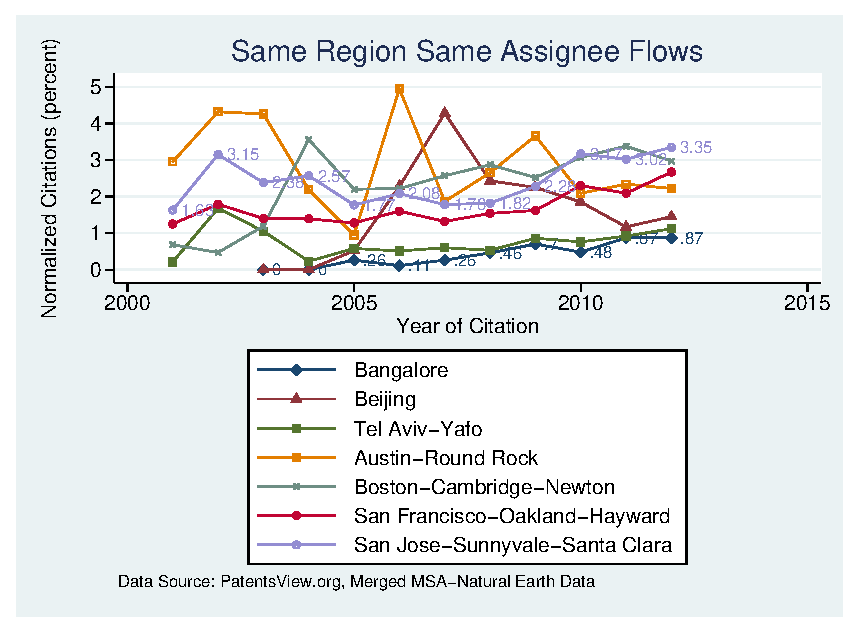
\includegraphics[width=\textwidth]{SameRegionSameAssigneeFlows}
  \caption{Local and Internal Flows by Region}
  \label{fig:SameRegionSameAssigneeFlows}
\end{centering}
\end{figure}

\begin{figure}[h]
\begin{centering}
  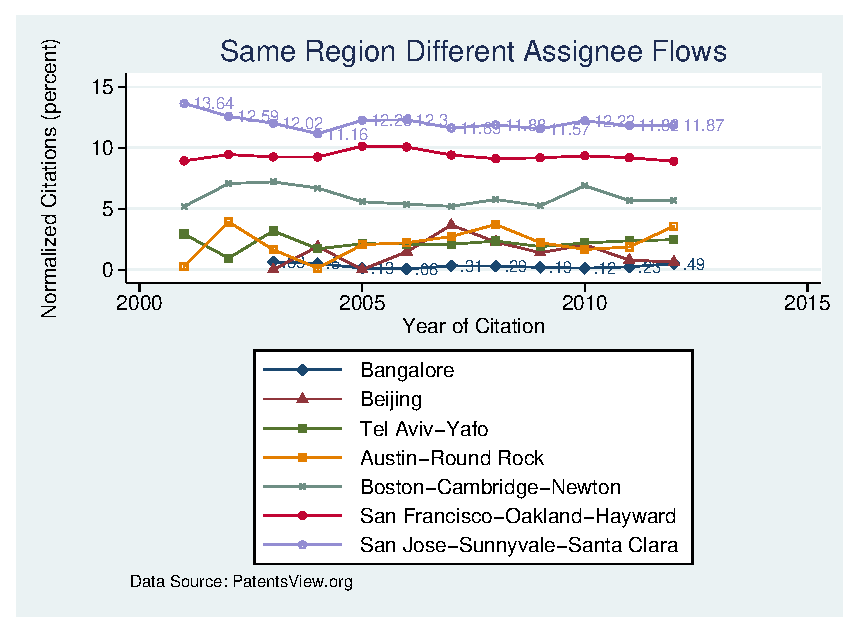
\includegraphics[width=\textwidth]{SameRegionDiffAssigneeFlows}
  \caption{Local and External Flows by Region}
  \label{fig:SameRegionDiffAssigneeFlows}
\end{centering}
\end{figure}


\begin{figure}[h]
\begin{centering}
  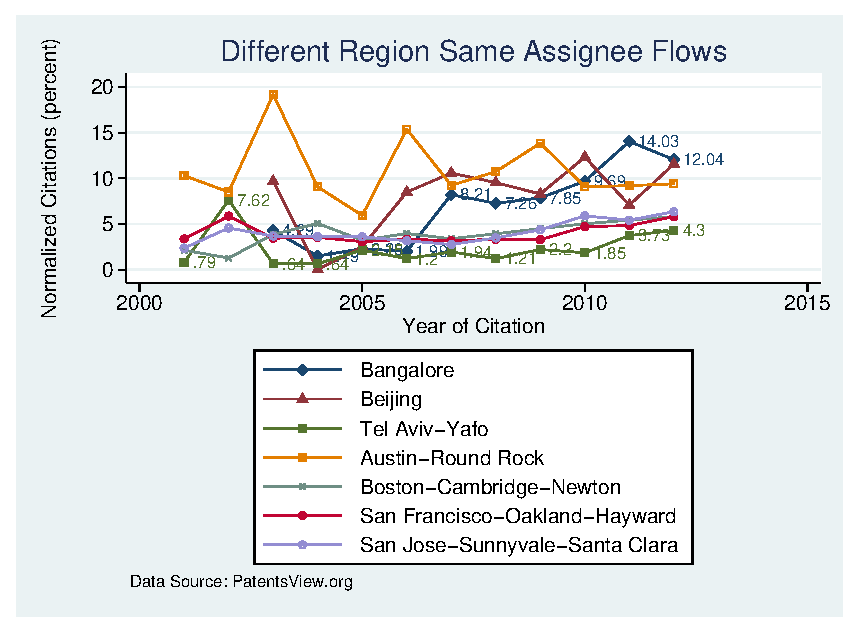
\includegraphics[width=\textwidth]{DiffRegionSameAssigneeFlows}
  \caption{Non-local and Internal Flows by Region}
  \label{fig:DiffRegionSameAssigneeFlows}
\end{centering}
\end{figure}

\begin{figure}[h]
\begin{centering}
  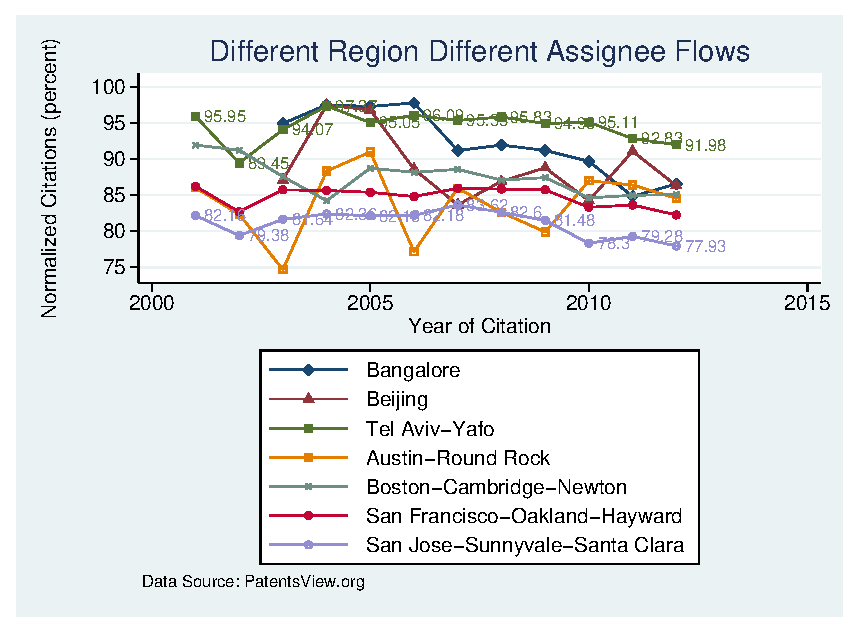
\includegraphics[width=\textwidth]{DiffRegionDiffAssigneeFlows}
  \caption{Non-local and External Flows by Region}
  \label{fig:DiffRegionDiffAssigneeFlows}
\end{centering}
\end{figure}

\section{Analysis of flows}\label{S:Analysis}
Table ~\ref{table:selected-citations} captures the number of citing patent-inventor-assignee to cited patent-inventor-assignee flows that form the dataset on which further investigation is conducted. Starting with 23,825,110 entries, we drop duplicate citations between the same patents and the same regions. This leaves us with 5,820,864 entries. In determining if the citing patent assignee and the cited patent assignee match, we drop all those entries where assignee information is unavailable for either side. That leaves us with  5,058,782 entries. We similarly drop those entries where either location region is unknown. We do so because it would seem incorrect to conclude that two locations differ when one location is undefined. After this step, we have 4,661,422 entries in our data set where conclusions can be clearly made about whether the assignees match and if the locations match between citing patent inventors and cited patent inventors. With this dataset, we calculate the normalized scores in our 2x2, and two aggregate measures - the first for same location flows across assignees, and the second for same assignee flows across locations. All six scores are expressed in percentages rounded to the nearest integer. The results are plotted in linear scale and are evident in the following graphs.
\newpage
\section{Preliminary Results}
Figure ~\ref{fig:SameRegionFlows} clearly indicates that the phenomenon of knowledge spillovers is strongly evident in the two California locations in our sample, and to a smaller extent in the extended Boston region. But clearly, the localization of knowledge spillovers is not observed in the three emerging country locations of Bangalore, Tel Aviv and Beijing. Figure {fig:SameRegionDiffAssigneeFlows} reiterates the gulf between the two California locations and the rest. On the other hand from Figure ~\ref{fig:SameAssigneeFlows}, we note that the Bangalore region has seen an increasing share of flows to non-local but internal flows. This maybe proof of an increasing amount of research being done in Bangalore by global multinationals for their corporate headquarters. It is also interesting to note that while Beijing and Bangalore are at a similar level (14 percent) in 2012 on this count, Bangalore has seen a steady increase while Beijing has somewhat stalled since 2005.
\\\\
Additionally, Figure ~\ref{fig:DiffRegionDiffAssigneeFlows} demonstrate the stark difference between Tel Aviv-Yafo and San Jose-Sunnyvale-Santa Clara, CA on the extent of non-local external flows. Tel Aviv-Yafo seems to be strongly integrated into the external knowledge network but not integrated much locally. Figure ~\ref{fig:DiffRegionSameAssigneeFlows} reiterates the Bangalore position as the outsourcing destination for global R\&D.
\newpage
\section{Main Results}

\begin{table}
\caption{Regression Results}
\begin{center}
\begin{tabular}{lccc}
\multicolumn{4}{c}{\begin{large}Effect of inventor resident regions on normalized aggregate local flows \label{local}\end{large}} \\ \hline
 & (1) & (2) & (3) \\
VARIABLES & Local Flows & Local Flows & Local Flows \\ \hline
\vspace{4pt} & \begin{footnotesize}\end{footnotesize} & \begin{footnotesize}\end{footnotesize} & \begin{footnotesize}\end{footnotesize} \\
Citing Region = Bangalore & -4.89*** & -4.89*** & -4.96*** \\
\vspace{4pt} & \begin{footnotesize}(0.00)\end{footnotesize} & \begin{footnotesize}(0.00)\end{footnotesize} & \begin{footnotesize}(0.00)\end{footnotesize} \\
Citing Region = Beijing & -2.54*** & -2.55*** & -2.52*** \\
\vspace{4pt} & \begin{footnotesize}(0.01)\end{footnotesize} & \begin{footnotesize}(0.01)\end{footnotesize} & \begin{footnotesize}(0.00)\end{footnotesize} \\
Citing Region = Boston & 4.40*** & 4.40*** & 4.42*** \\
\vspace{4pt} & \begin{footnotesize}(0.00)\end{footnotesize} & \begin{footnotesize}(0.00)\end{footnotesize} & \begin{footnotesize}(0.00)\end{footnotesize} \\
Citing Region = San Francisco & 6.70*** & 6.69*** & 6.76*** \\
\vspace{4pt} & \begin{footnotesize}(0.00)\end{footnotesize} & \begin{footnotesize}(0.00)\end{footnotesize} & \begin{footnotesize}(0.00)\end{footnotesize} \\
Citing Region = San Jose & 10.63*** & 10.63*** & 10.67*** \\
\vspace{4pt} & \begin{footnotesize}(0.00)\end{footnotesize} & \begin{footnotesize}(0.00)\end{footnotesize} & \begin{footnotesize}(0.00)\end{footnotesize} \\
Citing Region = Tel Aviv & -2.30*** & -2.30*** & -2.26*** \\
\vspace{4pt} & \begin{footnotesize}(0.00)\end{footnotesize} & \begin{footnotesize}(0.00)\end{footnotesize} & \begin{footnotesize}(0.00)\end{footnotesize} \\
Cited Region = Bangalore &  & 0.05*** & -0.00 \\
\vspace{4pt} & \begin{footnotesize}\end{footnotesize} & \begin{footnotesize}(0.01)\end{footnotesize} & \begin{footnotesize}(0.01)\end{footnotesize} \\
Cited Region = Beijing &  & 0.08*** & 0.06*** \\
\vspace{4pt} & \begin{footnotesize}\end{footnotesize} & \begin{footnotesize}(0.01)\end{footnotesize} & \begin{footnotesize}(0.01)\end{footnotesize} \\
Cited Region = Boston &  & 0.04*** & 0.02*** \\
\vspace{4pt} & \begin{footnotesize}\end{footnotesize} & \begin{footnotesize}(0.00)\end{footnotesize} & \begin{footnotesize}(0.00)\end{footnotesize} \\
Cited Region = San Francisco &  & 0.02*** & -0.00** \\
\vspace{4pt} & \begin{footnotesize}\end{footnotesize} & \begin{footnotesize}(0.00)\end{footnotesize} & \begin{footnotesize}(0.00)\end{footnotesize} \\
Cited Region = San Jose &  & 0.04*** & 0.01*** \\
\vspace{4pt} & \begin{footnotesize}\end{footnotesize} & \begin{footnotesize}(0.00)\end{footnotesize} & \begin{footnotesize}(0.00)\end{footnotesize} \\
Cited Region = Tel Aviv &  & 0.04*** & 0.01** \\
\vspace{4pt} & \begin{footnotesize}\end{footnotesize} & \begin{footnotesize}(0.00)\end{footnotesize} & \begin{footnotesize}(0.00)\end{footnotesize} \\
Constant & 5.97*** & 5.96*** & 7.93*** \\
 & \begin{footnotesize}(0.00)\end{footnotesize} & \begin{footnotesize}(0.00)\end{footnotesize} & \begin{footnotesize}(0.01)\end{footnotesize} \\
\vspace{4pt} & \begin{footnotesize}\end{footnotesize} & \begin{footnotesize}\end{footnotesize} & \begin{footnotesize}\end{footnotesize} \\
Observations & 4,660,110 & 4,660,110 & 4,660,110 \\
 $R^2$ & 0.95 & 0.95 & 0.98 \\ \hline
\multicolumn{4}{c}{\begin{footnotesize} Standard errors in parentheses\end{footnotesize}} \\
\multicolumn{4}{c}{\begin{footnotesize} Coefficient estimates relative to those for Austin\end{footnotesize}} \\
\multicolumn{4}{c}{\begin{footnotesize} Model 3 includes Year Fixed Effects\end{footnotesize}} \\
\multicolumn{4}{c}{\begin{footnotesize} *** p$<$0.01, ** p$<$0.05, * p$<$0.1\end{footnotesize}} \\
\end{tabular}
\end{center}

\end{table}

\begin{table}
\caption{Regression Results}
\begin{center}
\begin{tabular}{lccc}
\multicolumn{4}{c}{\begin{large}Effect of inventor resident regions on normalized aggregate internal flows \label{internal}\end{large}} \\ \hline
 & (1) & (2) & (3) \\
VARIABLES & Internal Flows & Internal Flows & Internal Flows \\ \hline
\vspace{4pt} & \begin{footnotesize}\end{footnotesize} & \begin{footnotesize}\end{footnotesize} & \begin{footnotesize}\end{footnotesize} \\
<<<<<<< HEAD
Citing Region = Bangalore & -2.52*** & -2.53*** & -2.53*** \\
\vspace{4pt} & \begin{footnotesize}(0.01)\end{footnotesize} & \begin{footnotesize}(0.01)\end{footnotesize} & \begin{footnotesize}(0.00)\end{footnotesize} \\
Citing Region = Beijing & -1.73*** & -1.74*** & -1.61*** \\
\vspace{4pt} & \begin{footnotesize}(0.02)\end{footnotesize} & \begin{footnotesize}(0.02)\end{footnotesize} & \begin{footnotesize}(0.01)\end{footnotesize} \\
Citing Region = Boston & -4.64*** & -4.64*** & -4.53*** \\
\vspace{4pt} & \begin{footnotesize}(0.01)\end{footnotesize} & \begin{footnotesize}(0.01)\end{footnotesize} & \begin{footnotesize}(0.00)\end{footnotesize} \\
Citing Region = San Francisco & -6.30*** & -6.30*** & -6.11*** \\
\vspace{4pt} & \begin{footnotesize}(0.01)\end{footnotesize} & \begin{footnotesize}(0.01)\end{footnotesize} & \begin{footnotesize}(0.00)\end{footnotesize} \\
Citing Region = San Jose & -4.74*** & -4.75*** & -4.66*** \\
\vspace{4pt} & \begin{footnotesize}(0.01)\end{footnotesize} & \begin{footnotesize}(0.01)\end{footnotesize} & \begin{footnotesize}(0.00)\end{footnotesize} \\
Citing Region = Tel Aviv & -10.28*** & -10.28*** & -10.03*** \\
\vspace{4pt} & \begin{footnotesize}(0.01)\end{footnotesize} & \begin{footnotesize}(0.01)\end{footnotesize} & \begin{footnotesize}(0.00)\end{footnotesize} \\
Cited Region = Bangalore &  & 0.35*** & 0.10*** \\
\vspace{4pt} & \begin{footnotesize}\end{footnotesize} & \begin{footnotesize}(0.03)\end{footnotesize} & \begin{footnotesize}(0.01)\end{footnotesize} \\
Cited Region = Beijing &  & 0.26*** & 0.13*** \\
\vspace{4pt} & \begin{footnotesize}\end{footnotesize} & \begin{footnotesize}(0.03)\end{footnotesize} & \begin{footnotesize}(0.01)\end{footnotesize} \\
Cited Region = Boston &  & 0.00 & -0.00** \\
\vspace{4pt} & \begin{footnotesize}\end{footnotesize} & \begin{footnotesize}(0.00)\end{footnotesize} & \begin{footnotesize}(0.00)\end{footnotesize} \\
Cited Region = San Francisco &  & 0.02*** & -0.00*** \\
\vspace{4pt} & \begin{footnotesize}\end{footnotesize} & \begin{footnotesize}(0.00)\end{footnotesize} & \begin{footnotesize}(0.00)\end{footnotesize} \\
Cited Region = San Jose &  & 0.08*** & 0.01*** \\
\vspace{4pt} & \begin{footnotesize}\end{footnotesize} & \begin{footnotesize}(0.00)\end{footnotesize} & \begin{footnotesize}(0.00)\end{footnotesize} \\
Cited Region = Tel Aviv &  & 0.11*** & -0.00 \\
\vspace{4pt} & \begin{footnotesize}\end{footnotesize} & \begin{footnotesize}(0.01)\end{footnotesize} & \begin{footnotesize}(0.00)\end{footnotesize} \\
Constant & 13.50*** & 13.49*** & 15.03*** \\
 & \begin{footnotesize}(0.01)\end{footnotesize} & \begin{footnotesize}(0.01)\end{footnotesize} & \begin{footnotesize}(0.01)\end{footnotesize} \\
\vspace{4pt} & \begin{footnotesize}\end{footnotesize} & \begin{footnotesize}\end{footnotesize} & \begin{footnotesize}\end{footnotesize} \\
Observations & 4,660,110 & 4,660,110 & 4,660,110 \\
 $R^2$ & 0.38 & 0.38 & 0.89 \\ \hline
\multicolumn{4}{c}{\begin{footnotesize} Standard errors in parentheses\end{footnotesize}} \\
=======
Citing Region = Bangalore & -2.45*** & -2.46*** & -2.49*** \\
\vspace{4pt} & \begin{footnotesize}(0.01)\end{footnotesize} & \begin{footnotesize}(0.01)\end{footnotesize} & \begin{footnotesize}(0.00)\end{footnotesize} \\
Citing Region = Beijing & -1.71*** & -1.71*** & -1.57*** \\
\vspace{4pt} & \begin{footnotesize}(0.02)\end{footnotesize} & \begin{footnotesize}(0.02)\end{footnotesize} & \begin{footnotesize}(0.01)\end{footnotesize} \\
Citing Region = Boston & -4.61*** & -4.61*** & -4.52*** \\
\vspace{4pt} & \begin{footnotesize}(0.01)\end{footnotesize} & \begin{footnotesize}(0.01)\end{footnotesize} & \begin{footnotesize}(0.00)\end{footnotesize} \\
Citing Region = San Francisco & -6.59*** & -6.59*** & -6.41*** \\
\vspace{4pt} & \begin{footnotesize}(0.01)\end{footnotesize} & \begin{footnotesize}(0.01)\end{footnotesize} & \begin{footnotesize}(0.00)\end{footnotesize} \\
Citing Region = San Jose & -4.78*** & -4.79*** & -4.71*** \\
\vspace{4pt} & \begin{footnotesize}(0.01)\end{footnotesize} & \begin{footnotesize}(0.01)\end{footnotesize} & \begin{footnotesize}(0.00)\end{footnotesize} \\
Citing Region = Tel Aviv & -10.69*** & -10.70*** & -10.46*** \\
\vspace{4pt} & \begin{footnotesize}(0.01)\end{footnotesize} & \begin{footnotesize}(0.01)\end{footnotesize} & \begin{footnotesize}(0.00)\end{footnotesize} \\
Cited Region = Bangalore &  & 0.36*** & 0.10*** \\
\vspace{4pt} & \begin{footnotesize}\end{footnotesize} & \begin{footnotesize}(0.03)\end{footnotesize} & \begin{footnotesize}(0.01)\end{footnotesize} \\
Cited Region = Beijing &  & 0.24*** & 0.13*** \\
\vspace{4pt} & \begin{footnotesize}\end{footnotesize} & \begin{footnotesize}(0.03)\end{footnotesize} & \begin{footnotesize}(0.01)\end{footnotesize} \\
Cited Region = Boston &  & 0.01** & -0.00 \\
\vspace{4pt} & \begin{footnotesize}\end{footnotesize} & \begin{footnotesize}(0.00)\end{footnotesize} & \begin{footnotesize}(0.00)\end{footnotesize} \\
Cited Region = San Francisco &  & 0.02*** & -0.01*** \\
\vspace{4pt} & \begin{footnotesize}\end{footnotesize} & \begin{footnotesize}(0.00)\end{footnotesize} & \begin{footnotesize}(0.00)\end{footnotesize} \\
Cited Region = San Jose &  & 0.08*** & 0.00*** \\
\vspace{4pt} & \begin{footnotesize}\end{footnotesize} & \begin{footnotesize}(0.00)\end{footnotesize} & \begin{footnotesize}(0.00)\end{footnotesize} \\
Cited Region = Tel Aviv &  & 0.11*** & -0.01* \\
\vspace{4pt} & \begin{footnotesize}\end{footnotesize} & \begin{footnotesize}(0.01)\end{footnotesize} & \begin{footnotesize}(0.00)\end{footnotesize} \\
Constant & 13.67*** & 13.66*** & 15.24*** \\
 & \begin{footnotesize}(0.01)\end{footnotesize} & \begin{footnotesize}(0.01)\end{footnotesize} & \begin{footnotesize}(0.01)\end{footnotesize} \\
\vspace{4pt} & \begin{footnotesize}\end{footnotesize} & \begin{footnotesize}\end{footnotesize} & \begin{footnotesize}\end{footnotesize} \\
Observations & 4,660,110 & 4,660,110 & 4,660,110 \\
 $R^2$ & 0.41 & 0.41 & 0.88 \\ \hline
\multicolumn{4}{c}{\begin{footnotesize} Standard errors in parentheses\end{footnotesize}} \\
\multicolumn{4}{c}{\begin{footnotesize} Coefficient estimates relative to those for Austin\end{footnotesize}} \\
\multicolumn{4}{c}{\begin{footnotesize} Model 3 includes Year Fixed Effects\end{footnotesize}} \\
>>>>>>> 569542730dc622482f425590d963455001b1940f
\multicolumn{4}{c}{\begin{footnotesize} *** p$<$0.01, ** p$<$0.05, * p$<$0.1\end{footnotesize}} \\
\end{tabular}
\end{center}

\end{table}

\begin{table}
\caption{Regression Results}
\begin{center}
\begin{tabular}{lccc}
\multicolumn{4}{c}{\begin{large}Effect of inventor resident regions on normalized aggregate local-internal flows \label{localinternal}\end{large}} \\ \hline
 & (1) & (2) & (3) \\
VARIABLES & Local-Internal & Local-Internal & Local-Internal \\ \hline
\vspace{4pt} & \begin{footnotesize}\end{footnotesize} & \begin{footnotesize}\end{footnotesize} & \begin{footnotesize}\end{footnotesize} \\
Citing Region = Bangalore & -2.30*** & -2.31*** & -2.34*** \\
\vspace{4pt} & \begin{footnotesize}(0.00)\end{footnotesize} & \begin{footnotesize}(0.00)\end{footnotesize} & \begin{footnotesize}(0.00)\end{footnotesize} \\
Citing Region = Beijing & -1.36*** & -1.36*** & -1.32*** \\
\vspace{4pt} & \begin{footnotesize}(0.01)\end{footnotesize} & \begin{footnotesize}(0.01)\end{footnotesize} & \begin{footnotesize}(0.00)\end{footnotesize} \\
Citing Region = Boston & 0.77*** & 0.77*** & 0.79*** \\
\vspace{4pt} & \begin{footnotesize}(0.00)\end{footnotesize} & \begin{footnotesize}(0.00)\end{footnotesize} & \begin{footnotesize}(0.00)\end{footnotesize} \\
Citing Region = San Francisco & -0.55*** & -0.56*** & -0.49*** \\
\vspace{4pt} & \begin{footnotesize}(0.00)\end{footnotesize} & \begin{footnotesize}(0.00)\end{footnotesize} & \begin{footnotesize}(0.00)\end{footnotesize} \\
Citing Region = San Jose & 0.29*** & 0.29*** & 0.31*** \\
\vspace{4pt} & \begin{footnotesize}(0.00)\end{footnotesize} & \begin{footnotesize}(0.00)\end{footnotesize} & \begin{footnotesize}(0.00)\end{footnotesize} \\
Citing Region = Tel Aviv & -2.15*** & -2.15*** & -2.09*** \\
\vspace{4pt} & \begin{footnotesize}(0.00)\end{footnotesize} & \begin{footnotesize}(0.00)\end{footnotesize} & \begin{footnotesize}(0.00)\end{footnotesize} \\
Cited Region = Bangalore &  & 0.06*** & -0.02*** \\
\vspace{4pt} & \begin{footnotesize}\end{footnotesize} & \begin{footnotesize}(0.01)\end{footnotesize} & \begin{footnotesize}(0.01)\end{footnotesize} \\
Cited Region = Beijing &  & 0.05*** & 0.02*** \\
\vspace{4pt} & \begin{footnotesize}\end{footnotesize} & \begin{footnotesize}(0.01)\end{footnotesize} & \begin{footnotesize}(0.01)\end{footnotesize} \\
Cited Region = Boston &  & 0.01*** & 0.00*** \\
\vspace{4pt} & \begin{footnotesize}\end{footnotesize} & \begin{footnotesize}(0.00)\end{footnotesize} & \begin{footnotesize}(0.00)\end{footnotesize} \\
Cited Region = San Francisco &  & 0.01*** & -0.00*** \\
\vspace{4pt} & \begin{footnotesize}\end{footnotesize} & \begin{footnotesize}(0.00)\end{footnotesize} & \begin{footnotesize}(0.00)\end{footnotesize} \\
Cited Region = San Jose &  & 0.03*** & 0.00*** \\
\vspace{4pt} & \begin{footnotesize}\end{footnotesize} & \begin{footnotesize}(0.00)\end{footnotesize} & \begin{footnotesize}(0.00)\end{footnotesize} \\
Cited Region = Tel Aviv &  & 0.03*** & -0.01*** \\
\vspace{4pt} & \begin{footnotesize}\end{footnotesize} & \begin{footnotesize}(0.00)\end{footnotesize} & \begin{footnotesize}(0.00)\end{footnotesize} \\
Constant & 3.14*** & 3.13*** & 4.18*** \\
 & \begin{footnotesize}(0.00)\end{footnotesize} & \begin{footnotesize}(0.00)\end{footnotesize} & \begin{footnotesize}(0.01)\end{footnotesize} \\
\vspace{4pt} & \begin{footnotesize}\end{footnotesize} & \begin{footnotesize}\end{footnotesize} & \begin{footnotesize}\end{footnotesize} \\
Observations & 4,660,110 & 4,660,110 & 4,660,110 \\
 $R^2$ & 0.52 & 0.52 & 0.86 \\ \hline
\multicolumn{4}{c}{\begin{footnotesize} Standard errors in parentheses\end{footnotesize}} \\
\multicolumn{4}{c}{\begin{footnotesize} Coefficient estimates relative to those for Austin\end{footnotesize}} \\
\multicolumn{4}{c}{\begin{footnotesize} Model 3 includes Year Fixed Effects\end{footnotesize}} \\
\multicolumn{4}{c}{\begin{footnotesize} *** p$<$0.01, ** p$<$0.05, * p$<$0.1\end{footnotesize}} \\
\end{tabular}
\end{center}


\end{table}

\begin{table}
\caption{Regression Results}
\begin{center}
\begin{tabular}{lccc}
\multicolumn{4}{c}{\begin{large}Effect of inventor resident regions on normalized aggregate local-external flows \label{localexternal}\end{large}} \\ \hline
 & (1) & (2) & (3) \\
VARIABLES & Local-External & Local-External & Local-External \\ \hline
\vspace{4pt} & \begin{footnotesize}\end{footnotesize} & \begin{footnotesize}\end{footnotesize} & \begin{footnotesize}\end{footnotesize} \\
Citing Region = Bangalore & -2.59*** & -2.59*** & -2.63*** \\
\vspace{4pt} & \begin{footnotesize}(0.00)\end{footnotesize} & \begin{footnotesize}(0.00)\end{footnotesize} & \begin{footnotesize}(0.00)\end{footnotesize} \\
Citing Region = Beijing & -1.18*** & -1.18*** & -1.21*** \\
\vspace{4pt} & \begin{footnotesize}(0.00)\end{footnotesize} & \begin{footnotesize}(0.00)\end{footnotesize} & \begin{footnotesize}(0.00)\end{footnotesize} \\
Citing Region = Boston & 3.63*** & 3.63*** & 3.63*** \\
\vspace{4pt} & \begin{footnotesize}(0.00)\end{footnotesize} & \begin{footnotesize}(0.00)\end{footnotesize} & \begin{footnotesize}(0.00)\end{footnotesize} \\
Citing Region = San Francisco & 7.25*** & 7.25*** & 7.25*** \\
\vspace{4pt} & \begin{footnotesize}(0.00)\end{footnotesize} & \begin{footnotesize}(0.00)\end{footnotesize} & \begin{footnotesize}(0.00)\end{footnotesize} \\
Citing Region = San Jose & 10.35*** & 10.34*** & 10.35*** \\
\vspace{4pt} & \begin{footnotesize}(0.00)\end{footnotesize} & \begin{footnotesize}(0.00)\end{footnotesize} & \begin{footnotesize}(0.00)\end{footnotesize} \\
Citing Region = Tel Aviv & -0.15*** & -0.15*** & -0.17*** \\
\vspace{4pt} & \begin{footnotesize}(0.00)\end{footnotesize} & \begin{footnotesize}(0.00)\end{footnotesize} & \begin{footnotesize}(0.00)\end{footnotesize} \\
Cited Region = Bangalore &  & -0.02** & 0.01** \\
\vspace{4pt} & \begin{footnotesize}\end{footnotesize} & \begin{footnotesize}(0.01)\end{footnotesize} & \begin{footnotesize}(0.01)\end{footnotesize} \\
Cited Region = Beijing &  & 0.04*** & 0.04*** \\
\vspace{4pt} & \begin{footnotesize}\end{footnotesize} & \begin{footnotesize}(0.01)\end{footnotesize} & \begin{footnotesize}(0.01)\end{footnotesize} \\
Cited Region = Boston &  & 0.02*** & 0.01*** \\
\vspace{4pt} & \begin{footnotesize}\end{footnotesize} & \begin{footnotesize}(0.00)\end{footnotesize} & \begin{footnotesize}(0.00)\end{footnotesize} \\
Cited Region = San Francisco &  & 0.01*** & 0.00** \\
\vspace{4pt} & \begin{footnotesize}\end{footnotesize} & \begin{footnotesize}(0.00)\end{footnotesize} & \begin{footnotesize}(0.00)\end{footnotesize} \\
Cited Region = San Jose &  & 0.01*** & 0.01*** \\
\vspace{4pt} & \begin{footnotesize}\end{footnotesize} & \begin{footnotesize}(0.00)\end{footnotesize} & \begin{footnotesize}(0.00)\end{footnotesize} \\
Cited Region = Tel Aviv &  & 0.01** & 0.01*** \\
\vspace{4pt} & \begin{footnotesize}\end{footnotesize} & \begin{footnotesize}(0.00)\end{footnotesize} & \begin{footnotesize}(0.00)\end{footnotesize} \\
Constant & 2.83*** & 2.83*** & 3.75*** \\
 & \begin{footnotesize}(0.00)\end{footnotesize} & \begin{footnotesize}(0.00)\end{footnotesize} & \begin{footnotesize}(0.01)\end{footnotesize} \\
\vspace{4pt} & \begin{footnotesize}\end{footnotesize} & \begin{footnotesize}\end{footnotesize} & \begin{footnotesize}\end{footnotesize} \\
Observations & 4,660,110 & 4,660,110 & 4,660,110 \\
 $R^2$ & 0.98 & 0.98 & 0.99 \\ \hline
\multicolumn{4}{c}{\begin{footnotesize} Standard errors in parentheses\end{footnotesize}} \\
\multicolumn{4}{c}{\begin{footnotesize} Coefficient estimates relative to those for Austin\end{footnotesize}} \\
\multicolumn{4}{c}{\begin{footnotesize} Model 3 includes Year Fixed Effects\end{footnotesize}} \\
\multicolumn{4}{c}{\begin{footnotesize} *** p$<$0.01, ** p$<$0.05, * p$<$0.1\end{footnotesize}} \\
\end{tabular}
\end{center}


\end{table}

\begin{table}
\caption{Regression Results}
\begin{center}
\begin{tabular}{lccc}
\multicolumn{4}{c}{\begin{large}Effect of inventor resident regions on normalized aggregate nonlocal-internal flows \label{nonlocalinternal}\end{large}} \\ \hline
 & (1) & (2) & (3) \\
VARIABLES & Non-Local-Internal & Non-Local-Internal & Non-Local-Internal \\ \hline
\vspace{4pt} & \begin{footnotesize}\end{footnotesize} & \begin{footnotesize}\end{footnotesize} & \begin{footnotesize}\end{footnotesize} \\
Citing Region = Bangalore & -0.15*** & -0.15*** & -0.15*** \\
\vspace{4pt} & \begin{footnotesize}(0.01)\end{footnotesize} & \begin{footnotesize}(0.01)\end{footnotesize} & \begin{footnotesize}(0.00)\end{footnotesize} \\
Citing Region = Beijing & -0.34*** & -0.35*** & -0.25*** \\
\vspace{4pt} & \begin{footnotesize}(0.01)\end{footnotesize} & \begin{footnotesize}(0.01)\end{footnotesize} & \begin{footnotesize}(0.01)\end{footnotesize} \\
Citing Region = Boston & -5.38*** & -5.38*** & -5.31*** \\
\vspace{4pt} & \begin{footnotesize}(0.01)\end{footnotesize} & \begin{footnotesize}(0.01)\end{footnotesize} & \begin{footnotesize}(0.00)\end{footnotesize} \\
Citing Region = San Francisco & -6.03*** & -6.04*** & -5.92*** \\
\vspace{4pt} & \begin{footnotesize}(0.00)\end{footnotesize} & \begin{footnotesize}(0.00)\end{footnotesize} & \begin{footnotesize}(0.00)\end{footnotesize} \\
Citing Region = San Jose & -5.07*** & -5.07*** & -5.02*** \\
\vspace{4pt} & \begin{footnotesize}(0.00)\end{footnotesize} & \begin{footnotesize}(0.00)\end{footnotesize} & \begin{footnotesize}(0.00)\end{footnotesize} \\
Citing Region = Tel Aviv & -8.54*** & -8.54*** & -8.37*** \\
\vspace{4pt} & \begin{footnotesize}(0.01)\end{footnotesize} & \begin{footnotesize}(0.01)\end{footnotesize} & \begin{footnotesize}(0.00)\end{footnotesize} \\
Cited Region = Bangalore &  & 0.30*** & 0.12*** \\
\vspace{4pt} & \begin{footnotesize}\end{footnotesize} & \begin{footnotesize}(0.02)\end{footnotesize} & \begin{footnotesize}(0.01)\end{footnotesize} \\
Cited Region = Beijing &  & 0.19*** & 0.11*** \\
\vspace{4pt} & \begin{footnotesize}\end{footnotesize} & \begin{footnotesize}(0.02)\end{footnotesize} & \begin{footnotesize}(0.01)\end{footnotesize} \\
Cited Region = Boston &  & -0.00 & -0.00*** \\
\vspace{4pt} & \begin{footnotesize}\end{footnotesize} & \begin{footnotesize}(0.00)\end{footnotesize} & \begin{footnotesize}(0.00)\end{footnotesize} \\
Cited Region = San Francisco &  & 0.01*** & -0.01*** \\
\vspace{4pt} & \begin{footnotesize}\end{footnotesize} & \begin{footnotesize}(0.00)\end{footnotesize} & \begin{footnotesize}(0.00)\end{footnotesize} \\
Cited Region = San Jose &  & 0.05*** & 0.00*** \\
\vspace{4pt} & \begin{footnotesize}\end{footnotesize} & \begin{footnotesize}(0.00)\end{footnotesize} & \begin{footnotesize}(0.00)\end{footnotesize} \\
Cited Region = Tel Aviv &  & 0.08*** & -0.00 \\
\vspace{4pt} & \begin{footnotesize}\end{footnotesize} & \begin{footnotesize}(0.01)\end{footnotesize} & \begin{footnotesize}(0.00)\end{footnotesize} \\
Constant & 10.53*** & 10.53*** & 11.06*** \\
 & \begin{footnotesize}(0.00)\end{footnotesize} & \begin{footnotesize}(0.00)\end{footnotesize} & \begin{footnotesize}(0.01)\end{footnotesize} \\
\vspace{4pt} & \begin{footnotesize}\end{footnotesize} & \begin{footnotesize}\end{footnotesize} & \begin{footnotesize}\end{footnotesize} \\
Observations & 4,660,110 & 4,660,110 & 4,660,110 \\
 $R^2$ & 0.46 & 0.46 & 0.87 \\ \hline
\multicolumn{4}{c}{\begin{footnotesize} Standard errors in parentheses\end{footnotesize}} \\
\multicolumn{4}{c}{\begin{footnotesize} Coefficient estimates relative to those for Austin\end{footnotesize}} \\
\multicolumn{4}{c}{\begin{footnotesize} Model 3 includes Year Fixed Effects\end{footnotesize}} \\
\multicolumn{4}{c}{\begin{footnotesize} *** p$<$0.01, ** p$<$0.05, * p$<$0.1\end{footnotesize}} \\
\end{tabular}
\end{center}


\end{table}

\begin{table}
\caption{Regression Results}
\begin{center}
\begin{tabular}{lccc}
\multicolumn{4}{c}{\begin{large}Effect of inventor resident regions on normalized aggregate nonlocal-external flows \label{nonlocalexternal}\end{large}} \\ \hline
 & (1) & (2) & (3) \\
VARIABLES & Non-Local-External & Non-Local-External & Non-Local-External \\ \hline
\vspace{4pt} & \begin{footnotesize}\end{footnotesize} & \begin{footnotesize}\end{footnotesize} & \begin{footnotesize}\end{footnotesize} \\
Citing Region = Bangalore & 5.03*** & 5.03*** & 5.08*** \\
\vspace{4pt} & \begin{footnotesize}(0.01)\end{footnotesize} & \begin{footnotesize}(0.01)\end{footnotesize} & \begin{footnotesize}(0.01)\end{footnotesize} \\
Citing Region = Beijing & 2.78*** & 2.79*** & 2.66*** \\
\vspace{4pt} & \begin{footnotesize}(0.02)\end{footnotesize} & \begin{footnotesize}(0.02)\end{footnotesize} & \begin{footnotesize}(0.01)\end{footnotesize} \\
Citing Region = Boston & 0.66*** & 0.66*** & 0.55*** \\
\vspace{4pt} & \begin{footnotesize}(0.01)\end{footnotesize} & \begin{footnotesize}(0.01)\end{footnotesize} & \begin{footnotesize}(0.00)\end{footnotesize} \\
Citing Region = San Francisco & -1.05*** & -1.04*** & -1.25*** \\
\vspace{4pt} & \begin{footnotesize}(0.01)\end{footnotesize} & \begin{footnotesize}(0.01)\end{footnotesize} & \begin{footnotesize}(0.00)\end{footnotesize} \\
Citing Region = San Jose & -5.58*** & -5.57*** & -5.67*** \\
\vspace{4pt} & \begin{footnotesize}(0.01)\end{footnotesize} & \begin{footnotesize}(0.01)\end{footnotesize} & \begin{footnotesize}(0.00)\end{footnotesize} \\
Citing Region = Tel Aviv & 10.58*** & 10.59*** & 10.34*** \\
\vspace{4pt} & \begin{footnotesize}(0.01)\end{footnotesize} & \begin{footnotesize}(0.01)\end{footnotesize} & \begin{footnotesize}(0.00)\end{footnotesize} \\
Cited Region = Bangalore &  & -0.34*** & -0.11*** \\
\vspace{4pt} & \begin{footnotesize}\end{footnotesize} & \begin{footnotesize}(0.03)\end{footnotesize} & \begin{footnotesize}(0.01)\end{footnotesize} \\
Cited Region = Beijing &  & -0.30*** & -0.18*** \\
\vspace{4pt} & \begin{footnotesize}\end{footnotesize} & \begin{footnotesize}(0.03)\end{footnotesize} & \begin{footnotesize}(0.01)\end{footnotesize} \\
Cited Region = Boston &  & -0.03*** & -0.01*** \\
\vspace{4pt} & \begin{footnotesize}\end{footnotesize} & \begin{footnotesize}(0.00)\end{footnotesize} & \begin{footnotesize}(0.00)\end{footnotesize} \\
Cited Region = San Francisco &  & -0.02*** & 0.01*** \\
\vspace{4pt} & \begin{footnotesize}\end{footnotesize} & \begin{footnotesize}(0.00)\end{footnotesize} & \begin{footnotesize}(0.00)\end{footnotesize} \\
Cited Region = San Jose &  & -0.09*** & -0.01*** \\
\vspace{4pt} & \begin{footnotesize}\end{footnotesize} & \begin{footnotesize}(0.00)\end{footnotesize} & \begin{footnotesize}(0.00)\end{footnotesize} \\
Cited Region = Tel Aviv &  & -0.11*** & -0.00 \\
\vspace{4pt} & \begin{footnotesize}\end{footnotesize} & \begin{footnotesize}(0.01)\end{footnotesize} & \begin{footnotesize}(0.01)\end{footnotesize} \\
Constant & 83.67*** & 83.68*** & 81.36*** \\
 & \begin{footnotesize}(0.01)\end{footnotesize} & \begin{footnotesize}(0.01)\end{footnotesize} & \begin{footnotesize}(0.01)\end{footnotesize} \\
\vspace{4pt} & \begin{footnotesize}\end{footnotesize} & \begin{footnotesize}\end{footnotesize} & \begin{footnotesize}\end{footnotesize} \\
Observations & 4,660,110 & 4,660,110 & 4,660,110 \\
 $R^2$ & 0.78 & 0.78 & 0.95 \\ \hline
\multicolumn{4}{c}{\begin{footnotesize} Standard errors in parentheses\end{footnotesize}} \\
\multicolumn{4}{c}{\begin{footnotesize} Coefficient estimates relative to those for Austin\end{footnotesize}} \\
\multicolumn{4}{c}{\begin{footnotesize} Model 3 includes Year Fixed Effects\end{footnotesize}} \\
\multicolumn{4}{c}{\begin{footnotesize} *** p$<$0.01, ** p$<$0.05, * p$<$0.1\end{footnotesize}} \\
\end{tabular}
\end{center}

\end{table}

We use inventor region dummy variables on an OLS regression on the normalized flows of knowledge to statistically substantiate the point we made graphically in our preliminary analysis. Tables ~\ref{local} to ~\ref{nonlocalexternal} capture the regression results corresponding to the six categories of flows we analyzed previously.
\\\\
At an aggregate level Table ~\ref{local} demonstrates that patents originating from the San Francisco and San Jose MSAs have a higher propensity for local knowledge flows. Bangalore, Beijing and Tel Aviv have the lowest local flows within the group, with Bangalore being the region with the lowest proportion of local flows.

Table ~\ref{internal} presents the aggregate level effect of region on internal (within firm) flows.  Here Austin (our base dummy) seems to do the best, with Tel Aviv being the region with the least internal flow. Bangalore and Beijing have internal flows higher than the San Francisco and San Jose MSAs, presumably reflecting the impact of multinationals. This is adequately supported in Table ~\ref{nonlocalinternal} where both Beijing and Bangalore have the highest coefficient estimates (after Austin) for the effect on non-local internal flows.

\section{Conclusion}
We started this article attempting to understand some of the factors that may explain the heterogeneity in knowledge flows across regions. While we have yet to get there, we have in the process demonstrated strong support for both the existence of the heterogeneity in knowledge flows across regions, as well as identifying some patterns relative to certain locations. We found that the San Francisco and San Jose MSA regions have the highest proportion of local knowledge flows, while Tel Aviv has the least. We also found that most of the flows for Tel Aviv patents are from different firms in different locations. Bangalore flows were higher to same firms in other locations, and were low to other firms locally. This study throws open opportunities to investigate specific mechanisms that might be leading to such behavior. While scholars have look at IPR regime effects, crossborder effects, we could consider looking at interconnectedness, modularity, and technology dynamics as potential explanatory variables in order to contribute to theory building on knowledge flows across locations.
\newpage


\begin{figure}[h]
\begin{centering}
  \includegraphics[width=\textwidth]{Austin}
  \caption{Geographic Definition of Austin-Round Rock, TX}
   \label{fig:Austin}
\end{centering}
\end{figure}

\begin{figure}[h]
\begin{centering}
  \includegraphics[width=\textwidth]{Bangalore}
  \caption{Geographic Definition of Bangalore}
   \label{fig:Bangalore}
\end{centering}
\end{figure}

\begin{figure}[h]
\begin{centering}
  \includegraphics[width=\textwidth]{Beijing}
  \caption{Geographic Definition of Beijing}
   \label{fig:Beijing}
\end{centering}
\end{figure}

\begin{figure}[h]
\begin{centering}
  \includegraphics[width=\textwidth]{Boston}
  \caption{Geographic Definition of Boston-Cambridge-Newton, MA-NH}
   \label{fig:Boston}
\end{centering}
\end{figure}

\begin{figure}[h]
\begin{centering}
  \includegraphics[width=\textwidth]{SanFrancisco}
  \caption{Geographic Definition of San Francisco-Oakland-Hayward, CA}
   \label{fig:SanFrancisco}
\end{centering}
\end{figure}

\begin{figure}[h]
\begin{centering}
  \includegraphics[width=\textwidth]{SanJose}
  \caption{Geographic Definition of San Jose-Sunnyvale-Santa Clara, CA}
   \label{fig:SanJose}
\end{centering}
\end{figure}

\begin{figure}[h]
\begin{centering}
  \includegraphics[width=\textwidth]{TelAviv}
  \caption{Geographic Definition of Tel Aviv-Yafo}
   \label{fig:TelAviv}
\end{centering}
\end{figure}


\bibliography{/Users/aiyenggar/OneDrive/code/bibliography/ae,/Users/aiyenggar/OneDrive/code/bibliography/fj,/Users/aiyenggar/OneDrive/code/bibliography/ko,/Users/aiyenggar/OneDrive/code/bibliography/pt,/Users/aiyenggar/OneDrive/code/bibliography/uz} 
\bibliographystyle{apalike}

\end{document}
